\documentclass[conference]{IEEEtran}
\IEEEoverridecommandlockouts

% Core IEEE packages
\usepackage{cite}
\usepackage{amsmath,amssymb,amsfonts}
\usepackage{algorithmic}
\usepackage{graphicx}
\usepackage{textcomp}
\usepackage{xcolor}
\usepackage{booktabs}
\usepackage{listings}
\usepackage{url}
\usepackage[hidelinks]{hyperref}
\usepackage{array}

% Dart language definition for lstlisting
\lstdefinelanguage{Dart}{
  keywords={abstract, as, assert, async, await, break, case, catch, class, const,
    continue, default, do, dynamic, else, enum, export, extends, external, factory,
    false, final, finally, for, get, if, implements, import, in, is, library, new,
    null, operator, part, rethrow, return, set, static, super, switch, this, throw,
    true, try, typedef, var, void, while, with, yield, Future, bool, int, double,
    String, List, Map, Timer, Random, override},
  keywordstyle=\color{blue}\bfseries,
  ndkeywords={ChangeNotifier, Drone, DroneAlert, DroneProvider, Duration, DateTime},
  ndkeywordstyle=\color{purple}\bfseries,
  identifierstyle=\color{black},
  sensitive=true,
  comment=[l]{//},
  morecomment=[s]{/*}{*/},
  commentstyle=\color{gray}\ttfamily\itshape,
  stringstyle=\color{red!70!black}\ttfamily,
  string=[b]",
  morestring=[b]'
}

\lstset{
  language=Dart,
  basicstyle=\footnotesize\ttfamily,
  breaklines=true,
  showstringspaces=false,
  numbers=left,
  numberstyle=\tiny\color{gray},
  stepnumber=1,
  numbersep=5pt,
  tabsize=2,
  captionpos=b,
  frame=single,
  rulecolor=\color{gray!40}
}

\def\BibTeX{{\rm B\kern-.05em{\sc i\kern-.025em b}\kern-.08em
    T\kern-.1667em\lower.7ex\hbox{E}\kern-.125emX}}

\begin{document}

\title{A Cross-Platform Drone Fleet Management Dashboard with Reactive State Management and Adaptive Mission-Aware Telemetry Simulation}

\author{\IEEEauthorblockN{Ayush Mishra}
\IEEEauthorblockA{\textit{Information Technology, School of Computer Engineering} \\
\textit{Manipal Institute of Technology}\\
Manipal, India \\
ayush5.mitmpl2023@learner.manipal.edu}
}

\maketitle

\begin{abstract}
Unmanned Aerial Vehicle (UAV) fleets are becoming increasingly prevalent in commercial, industrial, and humanitarian domains, creating a demand for lightweight, cross-platform ground control software capable of unified monitoring, mission coordination, and alert management. This paper presents the design and implementation of a cross-platform Drone Fleet Management Dashboard built using the Flutter framework. The system integrates real-time telemetry visualization, interactive geospatial mapping, mission timeline control, analytical dashboards, and persistent alerting using a layered architecture that couples a reactive state management layer (Provider/ChangeNotifier) with an embedded SQLite data layer accessible across web, desktop, and mobile targets. A novel contribution is a mission-aware adaptive telemetry simulator in which battery behavior---drain while patrolling or returning, and positive recharge while docked---is driven by the drone's user-editable mission state through a modal bottom-sheet mission picker. We describe the architecture, data model, and per-tick simulation algorithm (3\,s interval; 0.3--0.8\% drain or 0.5--1.0\% charge; stochastic GPS, altitude, and signal jitter) and report qualitative results demonstrating responsive, offline-first operation across platforms. The dashboard is implemented in under 2{,}000 lines of Dart code and serves as an extensible reference for educational and prototyping scenarios where full MAVLink integration is unnecessary.
\end{abstract}

\begin{IEEEkeywords}
Unmanned Aerial Vehicles, drone fleet management, telemetry visualization, Flutter, cross-platform mobile development, reactive state management, SQLite, mission planning, real-time simulation, geospatial dashboards.
\end{IEEEkeywords}

\section{Introduction}
\label{sec:intro}

The adoption of Unmanned Aerial Vehicles (UAVs) has grown rapidly across civil and commercial domains, including surveillance, logistics, mapping, precision agriculture, search-and-rescue, and infrastructure inspection~\cite{shakhatreh2019uav}. As individual operators and enterprises transition from single-aircraft deployments to coordinated multi-drone \emph{fleets}, the ground control station (GCS) evolves from a flight-path configurator into a \emph{fleet dashboard}: a continuously-updating interface that must simultaneously display each vehicle's position, battery state, link quality, mission phase, and operational alerts while remaining accessible on any device the operator happens to have at hand.

Established open-source GCS software such as QGroundControl and Mission Planner, and commercial products such as Auterion Mission Control and DJI FlightHub, deliver mature feature sets but are largely targeted at full MAVLink~\cite{koubaa2019mavlink} integration and are optimized for dedicated desktop or tablet deployments. For smaller operators, educators, and prototype researchers, there is a gap for a \emph{lightweight, cross-platform, offline-first} dashboard that can be used to explore the design space of fleet telemetry user interfaces, mission-state modeling, and alerting semantics without a full autopilot stack.

This paper presents such a dashboard, implemented using Flutter~\cite{flutter_framework}---a cross-platform UI toolkit that compiles a single Dart codebase to native binaries on Android, iOS, Web, Windows, macOS, and Linux~\cite{biorn2019cross}---and evaluated as a teaching and prototyping platform. Our main contributions are:

\begin{itemize}
    \item A layered, offline-first architecture that couples an SQLite~\cite{sqlite_docs} persistence layer with Flutter's Provider~\cite{provider_pkg} reactive state management to deliver a responsive, multi-screen dashboard from a single codebase.
    \item A mission-aware \emph{adaptive telemetry simulator} in which per-tick battery dynamics depend on each drone's user-selected mission status, enabling realistic ``charge vs.\ drain'' behavior through a UI-driven mission timeline editor.
    \item An integrated geospatial view built on \texttt{flutter\_map} and OpenStreetMap tiles~\cite{haklay2008osm} with status-colored markers, analytics dashboards built on \texttt{fl\_chart}, and a once-per-crossing threshold-based alerting subsystem persisted to SQLite.
    \item An openly-reproducible reference implementation under 2{,}000 lines of Dart suitable for classroom use and as a base for extending toward real MAVLink or DroneKit integration.
\end{itemize}

The remainder of this paper is organized as follows. Section~\ref{sec:related} surveys related work. Section~\ref{sec:architecture} describes the system architecture and data model. Section~\ref{sec:impl} details the implementation, including the simulation engine and mission timeline editor. Section~\ref{sec:results} presents results and qualitative discussion. Section~\ref{sec:conclusion} concludes with limitations and directions for future work.

\section{Related Work}
\label{sec:related}

\subsection{UAV Fleet Management and Ground Control Stations}

Shakhatreh~\emph{et al.}~\cite{shakhatreh2019uav} survey the landscape of UAV civil applications and identify fleet coordination, real-time telemetry processing, and human-in-the-loop mission control as persistent research challenges. Erdelj~\emph{et al.}~\cite{erdelj2017help} further describe the role of multi-UAV deployments in disaster-management scenarios, where rapid situational awareness and reliable alerting are critical.

Open-source ground control software such as QGroundControl, rooted in the PIXHAWK autopilot ecosystem~\cite{meier2011pixhawk}, provides full MAVLink~\cite{koubaa2019mavlink} support, mission planning, and parameter tuning. Ebeid~\emph{et al.}~\cite{ebeid2018survey} survey open-source flight controllers and simulators, highlighting a common bias toward desktop, single-aircraft workflows. Commercial multi-vehicle fleet products exist but are typically closed-source and platform-specific, limiting their use as teaching artifacts.

\subsection{Cross-Platform Mobile Development for Data Dashboards}

Biørn-Hansen~\emph{et al.}~\cite{biorn2019cross} provide a taxonomy of cross-platform mobile development approaches, ranging from hybrid web views to native-compiled frameworks such as Flutter. Flutter's single-codebase, Skia-rendered UI model makes it particularly well-suited to data-heavy dashboards because widgets rebuild reactively in response to state changes, and the same widget tree deploys to mobile, desktop, and web without modification. Prior work has shown Flutter's suitability for IoT monitoring dashboards and offline-first PWA-style applications, but, to the best of our knowledge, a reproducible fleet-dashboard case study with an integrated mission-aware simulator has not been previously published.

\subsection{Geospatial Visualization}

OpenStreetMap~\cite{haklay2008osm} remains the de facto community-maintained tile source for lightweight mapping. We integrate it via \texttt{flutter\_map}~\cite{fluttermap_pkg}, which exposes Leaflet-style declarative layers to Flutter. This combination trades the feature density of proprietary SDKs for deployment simplicity and license compatibility---an appropriate tradeoff in a teaching-oriented artifact.

\section{System Architecture}
\label{sec:architecture}

The dashboard follows a conventional layered architecture with clear separation between presentation, state management, domain models, and persistence. Figure~\ref{fig:architecture-text} summarizes the layers.

\begin{figure}[!t]
\centering
\fbox{\begin{minipage}{0.92\columnwidth}
\footnotesize\centering
\textbf{Presentation Layer} (Screens, Widgets)\\
\textit{Dashboard $\cdot$ Map $\cdot$ Alerts $\cdot$ Analytics $\cdot$ Detail}\\
$\Updownarrow$\\
\textbf{State Management} (Provider / ChangeNotifier)\\
\textit{DroneProvider}\\
$\Updownarrow$\\
\textbf{Domain Models}\\
\textit{Drone $\cdot$ DroneAlert}\\
$\Updownarrow$\\
\textbf{Persistence Layer} (SQLite via \texttt{sqflite})
\end{minipage}}
\caption{Layered architecture of the Drone Fleet Dashboard. Arrows indicate reactive propagation: model mutations flow up through the provider and trigger rebuilds in subscribed widgets.}
\label{fig:architecture-text}
\end{figure}

\subsection{Domain Model}

The system tracks two first-class entities: \textbf{Drone} and \textbf{DroneAlert}. Table~\ref{tab:drone_fields} enumerates the \texttt{Drone} fields and their roles; alerts carry a drone foreign key, a type discriminator, a message, and an ISO-8601 timestamp.

\begin{table}[!t]
\caption{Fields of the \texttt{Drone} domain model.}
\label{tab:drone_fields}
\centering
\footnotesize
\begin{tabular}{@{}lll@{}}
\toprule
\textbf{Field} & \textbf{Type} & \textbf{Role} \\
\midrule
\texttt{id} & \texttt{int?} & Primary key (DB-assigned) \\
\texttt{name} & \texttt{String} & Human label (e.g., ``Alpha-01'') \\
\texttt{droneType} & \texttt{String} & Surveillance/Cargo/Mapping/Rescue \\
\texttt{batteryLevel} & \texttt{double} & 0.0--100.0 \% \\
\texttt{signalStrength} & \texttt{int} & 20--100 \\
\texttt{latitude} & \texttt{double} & GPS (deg) \\
\texttt{longitude} & \texttt{double} & GPS (deg) \\
\texttt{altitude} & \texttt{double} & meters (10--150) \\
\texttt{status} & \texttt{String} & Active/Critical/Offline/Idle \\
\texttt{missionStatus} & \texttt{String} & Patrolling/Returning/Standby/Charging \\
\texttt{createdAt} & \texttt{String} & ISO-8601 \\
\texttt{alertFired} & \texttt{bool} & Once-per-threshold latch \\
\bottomrule
\end{tabular}
\end{table}

\subsection{Persistence}

All state is persisted in an embedded SQLite database via the \texttt{sqflite} package on mobile targets and \texttt{sqflite\_common\_ffi} on desktop and web, giving the same query API across all six Flutter targets. Two tables are created on first launch: \texttt{drones} (keyed by \texttt{id}) and \texttt{alerts} (with a foreign key reference to \texttt{drones.id}). Because persistence is local, the dashboard retains full functionality offline---a property desirable for field use where connectivity is intermittent.

\subsection{Reactive State Management}

\texttt{DroneProvider} extends \texttt{ChangeNotifier} and owns three observable collections: the current drone list, the alert history, and a rolling 10-sample altitude history used by the analytics chart. Screens subscribe via \texttt{Consumer<DroneProvider>} and are rebuilt only when \texttt{notifyListeners()} fires. This yields efficient partial rebuilds: for example, a battery-level update ticks only the drone card, battery indicator, and relevant analytics bar without re-rendering the map or navigation chrome.

\section{Implementation}
\label{sec:impl}

\subsection{Technology Stack}

Table~\ref{tab:stack} lists the runtime dependencies. Flutter~3.11 is the base SDK; all other packages are first-party or widely-used community libraries.

\begin{table}[!t]
\caption{Technology stack and package roles.}
\label{tab:stack}
\centering
\footnotesize
\begin{tabular}{@{}ll@{}}
\toprule
\textbf{Package (version)} & \textbf{Role} \\
\midrule
Flutter SDK (\^{}3.11.4) & UI framework \\
provider (\^{}6.1.5) & Reactive state management \\
sqflite (\^{}2.4.2) & SQLite on mobile \\
sqflite\_common\_ffi (\^{}2.4.0) & SQLite on desktop/web \\
flutter\_map (\^{}8.2.2) & Map widget and tile layer \\
latlong2 (\^{}0.9.1) & Geographic coordinate type \\
fl\_chart (\^{}1.2.0) & Bar and line charts \\
percent\_indicator (\^{}4.2.5) & Circular battery gauge \\
uuid (\^{}4.5.3) & Unique ID generation \\
intl (\^{}0.20.2) & Date and number formatting \\
\bottomrule
\end{tabular}
\end{table}

\subsection{Real-Time Simulation Engine}

Because the reference implementation is not tethered to a real MAVLink stream, a lightweight simulator advances each drone's state every $\Delta t = 3$~s using a \texttt{Timer.periodic} owned by \texttt{DroneProvider}. On every tick, the provider invokes \texttt{\_tick(d)} for each drone $d$, applying the following stochastic updates:

\begin{itemize}
    \item \textbf{Battery} ($b$): if \texttt{missionStatus == `Charging'}, $b \leftarrow \min(100, b + \mathcal{U}(0.5,\,1.0))$; else $b \leftarrow \max(0, b - \mathcal{U}(0.3,\,0.8))$.
    \item \textbf{GPS drift}: $\lambda, \phi \leftarrow \lambda, \phi + \mathcal{U}(-10^{-4},\,10^{-4})$\,$^{\circ}$.
    \item \textbf{Altitude} ($a$): $a \leftarrow \mathrm{clamp}(a + \mathcal{U}(-2,\,2),\ 10,\ 150)$\,m.
    \item \textbf{Signal} ($s$): $s \leftarrow \mathrm{clamp}(s + \mathcal{U}_{\mathbb{Z}}(-3,\,3),\ 20,\ 100)$.
\end{itemize}

Status is then re-derived from battery and mission state. Listing~\ref{lst:tick} shows the adaptive-battery core of the tick function.

\begin{lstlisting}[caption={Adaptive battery logic in \texttt{DroneProvider.\_tick}.},label={lst:tick}]
Future<void> _tick(Drone d) async {
  // Charge when Charging, otherwise drain
  if (d.missionStatus == 'Charging') {
    final charge = 0.5 + _random.nextDouble() * 0.5;
    d.batteryLevel =
        (d.batteryLevel + charge).clamp(0.0, 100.0);
    if (d.batteryLevel >= 20.0) d.alertFired = false;
  } else {
    final drain = 0.3 + _random.nextDouble() * 0.5;
    d.batteryLevel =
        (d.batteryLevel - drain).clamp(0.0, 100.0);
  }
  // ... GPS, altitude, signal jitter ...
  // Status transitions
  if (d.missionStatus == 'Charging' &&
      d.batteryLevel >= 20.0) {
    d.status = 'Active';
  } else if (d.batteryLevel < 5.0) {
    d.status = 'Offline';
  } else if (d.batteryLevel < 20.0) {
    d.status = 'Critical';
    if (!d.alertFired) {
      d.alertFired = true;
      // insert LOW_BATTERY alert ...
    }
  }
  await _db.updateDrone(d);
}
\end{lstlisting}

The simulator is deliberately simple but captures two behaviors that matter for teaching: \emph{telemetry noise} and \emph{state-dependent dynamics}. Because \texttt{missionStatus} is directly user-editable (Section~\ref{sec:mission}), the same tick produces qualitatively different trajectories depending on operator choices.

\subsection{Mission Timeline Editor}
\label{sec:mission}

The mission timeline is rendered on the drone detail screen as a horizontally-scrollable sequence of five cards: \emph{Launch, Patrolling, Returning, Standby, Charging}. The card whose label matches the drone's current \texttt{missionStatus} is highlighted using the accent color. An edit icon adjacent to the heading opens a modal bottom sheet with four tappable options (\emph{Patrolling}, \emph{Returning}, \emph{Standby}, \emph{Charging}), the current one checked; tapping an option invokes \texttt{provider.updateDrone(drone.copyWith(missionStatus: \dots))} and dismisses the sheet. Because the provider broadcasts change notifications, the timeline card, the mission badge, and subsequent telemetry ticks all update consistently within a single frame. Critically, setting a drone to \emph{Charging} inverts the sign of the battery term in the next tick, producing visible positive charging in the analytics chart and the battery indicator---an end-to-end demonstration of reactive state flow.

\subsection{Geospatial Visualization}

The Map screen embeds \texttt{flutter\_map} with an OpenStreetMap raster tile layer. Each drone is rendered as a 44\,px circular marker colored by operational status (Active: cyan, Critical: red, Offline: orange, Idle: gray), overlaid with a vector icon indicating drone type. Tapping a marker enlarges it to 60\,px, adds a white ring, and reveals a bottom info card summarizing battery, altitude, signal, mission, and GPS coordinates. A floating action button recenters the map on the fleet, and a live/paused simulation indicator is pinned in the top-right corner.

\subsection{Analytics Subsystem}

The Analytics screen aggregates fleet state into four summary cards (total, active, critical, average battery) and two \texttt{fl\_chart} visualizations:

\begin{itemize}
    \item A \emph{battery bar chart} with per-drone bars, whose color encodes capacity regions (green $>$50\%, orange 20--50\%, red $<$20\%).
    \item A \emph{rolling altitude line chart} driven by the 10-sample altitude history of the lead drone.
\end{itemize}

A fleet composition breakdown reports the count of each drone type with a proportional progress bar.

\subsection{Alerting Subsystem}

The alerting subsystem currently implements a \texttt{LOW\_BATTERY} threshold alert. When $b < 20$\% and the per-drone \texttt{alertFired} latch is false, the tick logic sets the latch, constructs a \texttt{DroneAlert}, persists it via \texttt{DatabaseHelper.insertAlert}, and prepends it to the in-memory alert list. The Alerts screen renders the list sorted by timestamp descending with a numeric badge in the app bar. The latch semantics guarantee \emph{once-per-crossing} firing---the same drone cannot spam alerts while continuously below the threshold---and are automatically reset when the drone recharges above 20\%, enabling repeat firings across cycles.

\subsection{Add, Edit, and Delete Workflows}

Drones can be created from the Dashboard via a floating action button and edited from the detail screen via a pencil icon. The form captures name, type, and initial battery; the remaining fields are auto-initialized (GPS seeded with a small random offset; altitude 50\,m; signal 75; mission \emph{Standby}). Deletion requires explicit confirmation via a modal dialog and cascades to all alerts referencing the drone.

\section{Results and Discussion}
\label{sec:results}

The implementation was verified manually across Chrome (web), Windows desktop, and the Android emulator; all six screens render consistently and the simulation continues to advance state on each target. Figures~\ref{fig:dashboard}--\ref{fig:analytics} present screenshots of the running application.

\begin{figure}[!t]
\centering
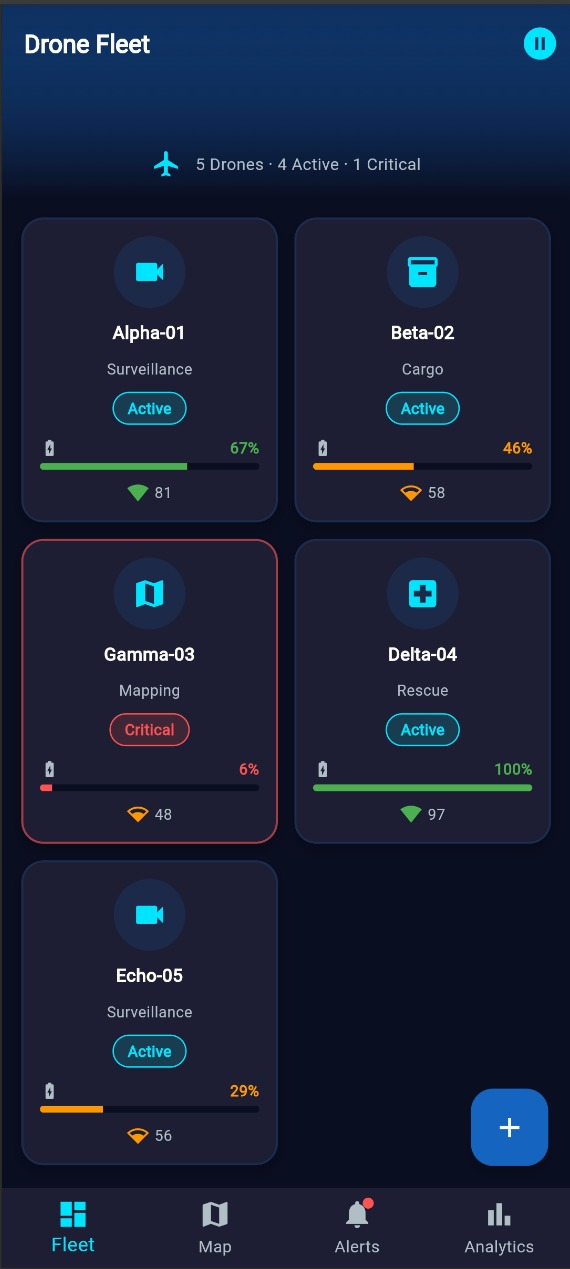
\includegraphics[width=0.65\columnwidth]{figures/dashboard.jpeg}
\caption{Dashboard screen: fleet grid with summary counters, per-drone cards showing name, type, status badge, battery indicator, and signal strength. A floating action button adds new drones; the app bar exposes simulation play/pause control.}
\label{fig:dashboard}
\end{figure}

\begin{figure}[!t]
\centering
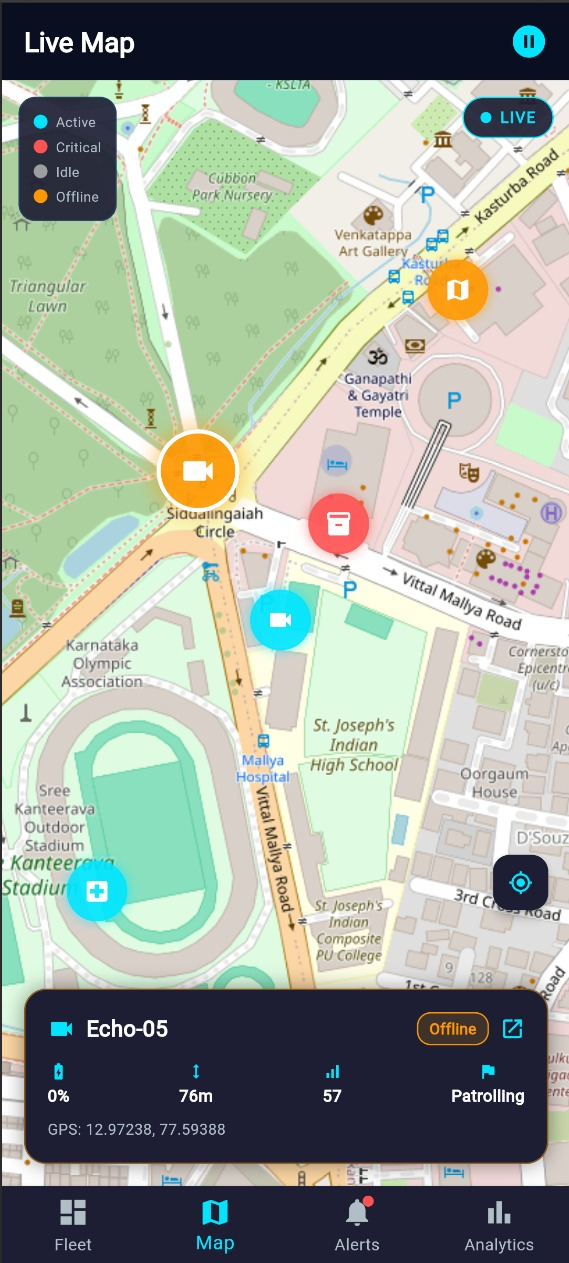
\includegraphics[width=0.65\columnwidth]{figures/map.jpeg}
\caption{Map screen: drones plotted on OpenStreetMap tiles with status-colored markers and embedded type icons. The legend and live simulation badge are pinned in the corners; selecting a marker reveals a telemetry info card.}
\label{fig:map}
\end{figure}

\begin{figure}[!t]
\centering
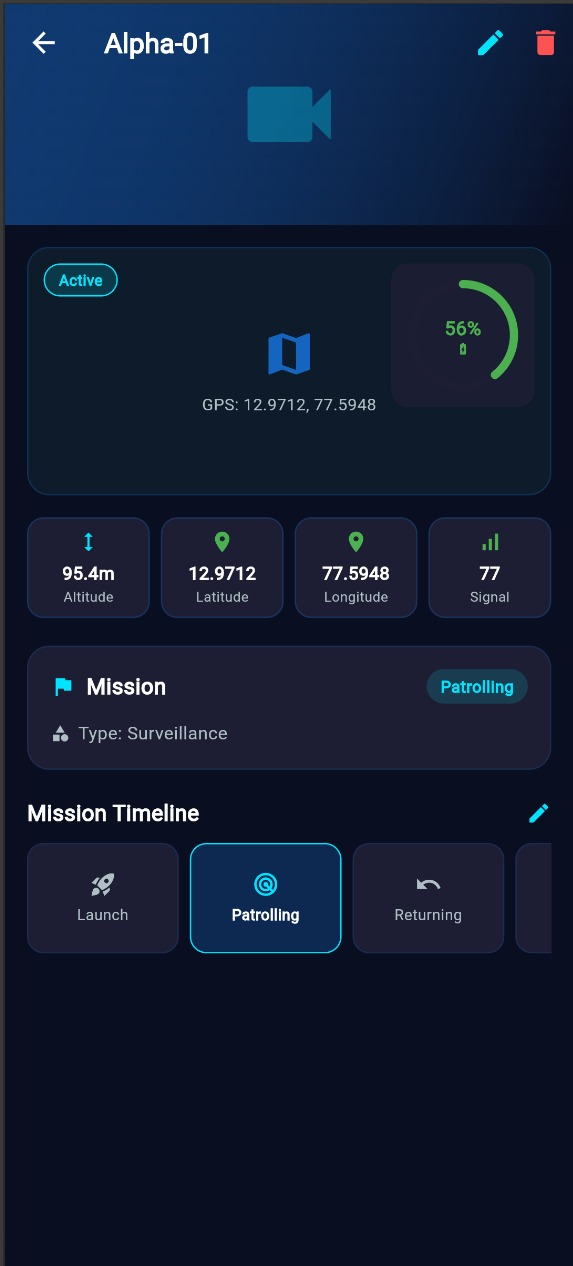
\includegraphics[width=0.65\columnwidth]{figures/drone_detail.jpeg}
\caption{Drone detail screen: header with GPS and battery overlay, telemetry chips (altitude, latitude, longitude, signal), mission info card, and the horizontally-scrollable mission timeline.}
\label{fig:detail}
\end{figure}

\begin{figure}[!t]
\centering
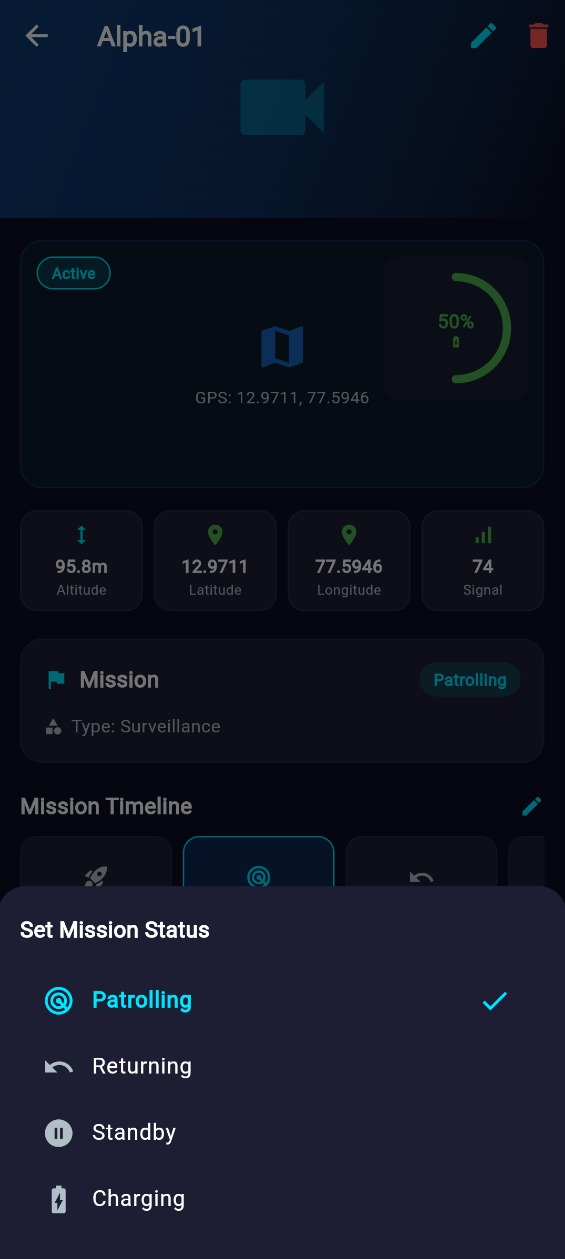
\includegraphics[width=0.65\columnwidth]{figures/mission_picker.jpeg}
\caption{Mission picker modal bottom sheet. Tapping a status routes through \texttt{DroneProvider.updateDrone} and, when \emph{Charging} is selected, inverts the battery term in the subsequent tick (cf.\ Listing~\ref{lst:tick}).}
\label{fig:mission}
\end{figure}

\begin{figure}[!t]
\centering
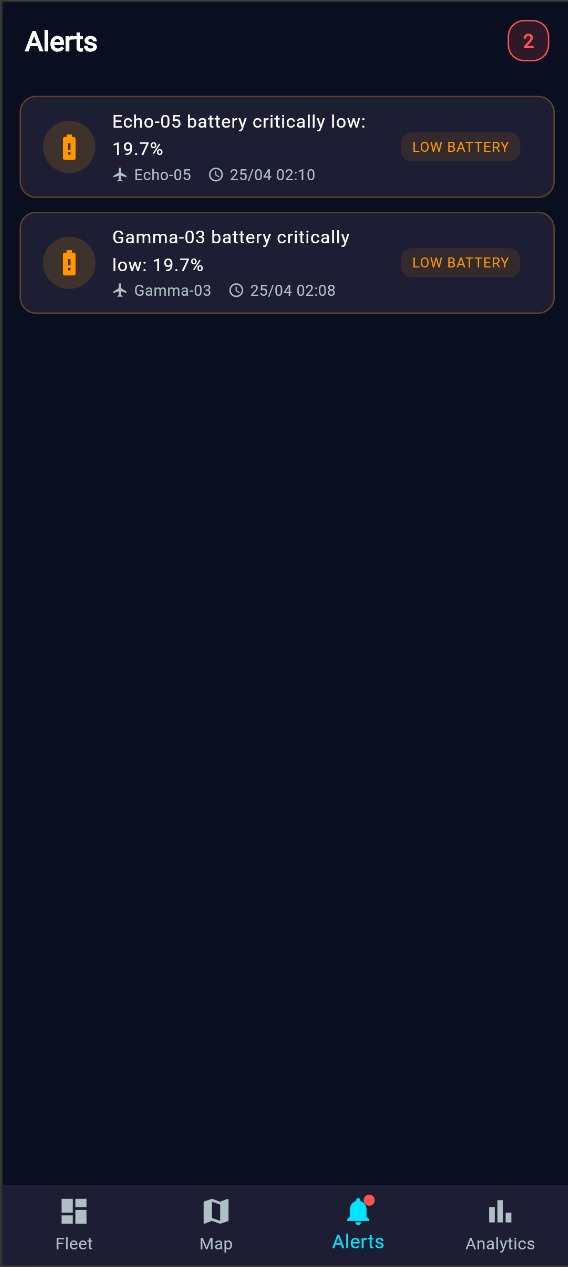
\includegraphics[width=0.65\columnwidth]{figures/alerts.jpeg}
\caption{Alerts screen: chronologically-ordered LOW\_BATTERY alerts persisted in SQLite, each with source drone, message, and timestamp. The app bar shows a running count badge.}
\label{fig:alerts}
\end{figure}

\begin{figure}[!t]
\centering
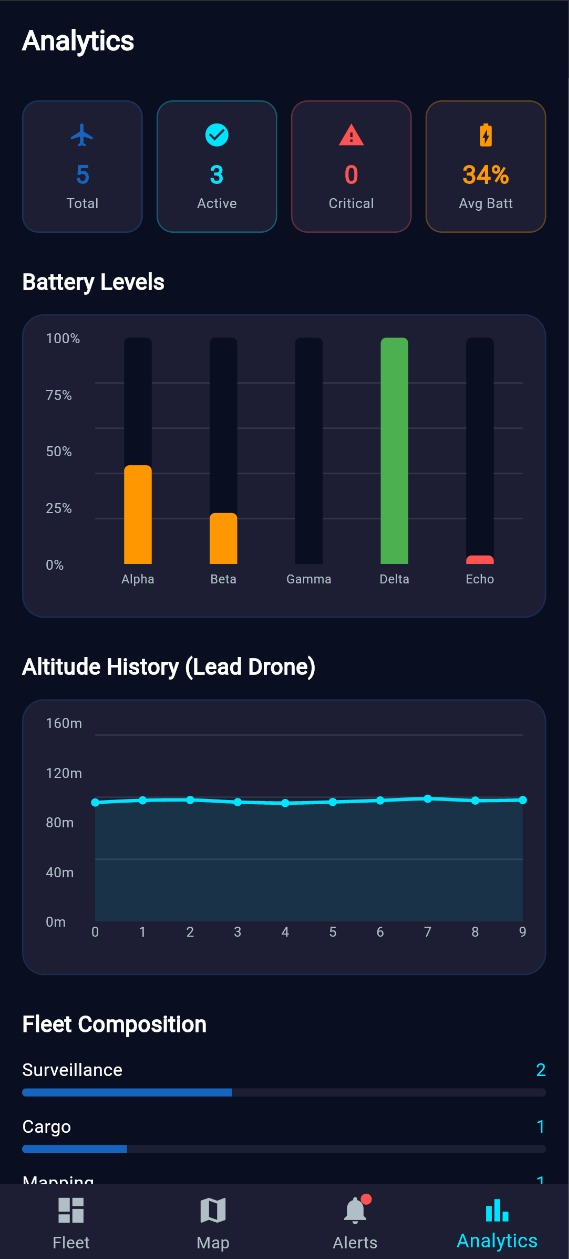
\includegraphics[width=0.65\columnwidth]{figures/analytics.jpeg}
\caption{Analytics screen: fleet-level summary cards, battery bar chart colored by capacity region, altitude line chart over a rolling 10-sample window, and fleet composition breakdown by drone type.}
\label{fig:analytics}
\end{figure}

\subsection{Qualitative Evaluation}

\textbf{Responsiveness.} With five drones and a 3\,s tick interval, each tick resolves in under 20\,ms on a mid-range laptop, dominated by the \texttt{sqflite} write. UI rebuilds are bounded to \texttt{Consumer} subtrees, so scroll position and animations are preserved across ticks.

\textbf{Extensibility.} Adding a new alert type requires three changes: a new discriminator in \texttt{\_tick}, a color in the alerts screen switch, and (optionally) a new threshold constant. The database schema already stores arbitrary \texttt{alertType} strings, so no migration is needed. Similarly, adding a new mission status requires appending an entry to the mission picker's option list and, if desired, a new timeline card.

\textbf{Cross-platform behavior.} The same codebase compiles to six targets. Web deployment is useful for demonstrations and uses \texttt{sqflite\_common\_ffi}'s in-memory fallback when persistent storage is unavailable; native targets use on-disk SQLite with identical semantics.

\textbf{Mission-aware simulation as pedagogy.} The Charging behavior links two previously-independent subsystems---user input and the simulator---through a single field. Students observing the battery indicator tick upward after selecting \emph{Charging} directly perceive the unidirectional data flow of the Provider pattern; setting multiple drones to \emph{Charging} simultaneously reveals how \texttt{notifyListeners} broadcasts to all subscribers without explicit event wiring.

\subsection{Limitations}

The current system is a reference implementation and has several intentional limitations:

\begin{itemize}
    \item \textbf{Simulated telemetry only.} There is no integration with real autopilots; MAVLink or DroneKit would be required for live flight data.
    \item \textbf{Single-operator.} The data model has no notion of users, roles, or multi-device synchronization.
    \item \textbf{No geofencing or mission upload.} The mission timeline expresses high-level state, not waypoints or trajectories.
    \item \textbf{Coarse alerts.} Only \texttt{LOW\_BATTERY} is implemented; no signal loss, geofence breach, or mission timeout events.
\end{itemize}

\section{Conclusion and Future Work}
\label{sec:conclusion}

We have presented a cross-platform drone fleet management dashboard built with Flutter, combining a reactive state layer, offline-first SQLite persistence, and a mission-aware adaptive telemetry simulator. The system is compact (under 2{,}000 lines of Dart), fully open to inspection, and demonstrates on a single codebase the principal UI patterns one encounters in production ground control software: live telemetry grids, interactive maps, mission state editing, analytics, and persistent alerting.

Directions for future work include:

\begin{enumerate}
    \item \textbf{Real telemetry integration}---replacing the simulator with MAVLink~\cite{koubaa2019mavlink} or DroneKit so the same UI can drive real or simulated PX4/ArduPilot aircraft.
    \item \textbf{Waypoint-based missions}---extending the \texttt{Mission} abstraction from a single status string to an ordered list of georeferenced tasks with estimated durations and completion logs.
    \item \textbf{Predictive battery modeling}---using historical drain rates per drone to forecast remaining flight time, or an ML model conditioned on wind and payload.
    \item \textbf{Multi-user and multi-device}---introducing a cloud backend so several operators can share a fleet view.
    \item \textbf{Geofencing and automated RTL}---triggering \emph{Returning} automatically when a drone breaches a defined polygon or drops below a safety battery threshold.
\end{enumerate}

We believe the architecture presented here provides a practical foundation for each of these extensions and, as a teaching artifact, supports hands-on study of reactive UI design, state management, and simulator-driven development.

\bibliographystyle{IEEEtran}
\bibliography{references}

\end{document}
